\documentclass[residuals.tex]{subfiles}
\Large
\begin{document}
\newpage
\Large
\section{Some Important Definitions}
\subsection{Homoscedasticity}
\begin{itemize}
\item \textbf{\textit{Homoscedascity}} is the technical term to describe the variance of the residuals being constant across the range of predicted values. 

\item \textbf{\textit{Heteroscedascity}} is the converse scenario : the variance differs along the range of values.
\end{itemize}


\noindent Suppose you plot the individual residuals against the predicted value, the variance of the residuals predicted value should be constant. 

\noindent Consider the red arrows in the picture below, intended to indicate the variance of the residuals at that part of the number line. For the OLS summption to be valid , the length of the red lines should be more or less the same.

\begin{figure}[h!]
\centering
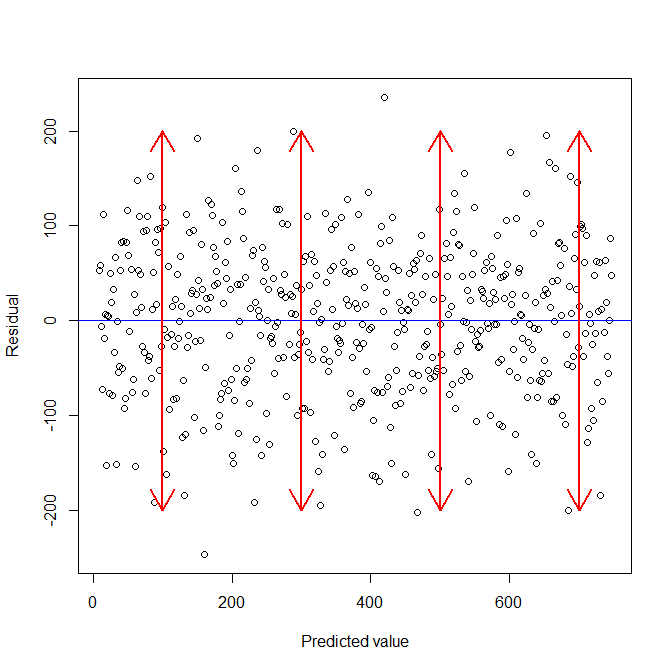
\includegraphics[width=0.6\linewidth]{homosked}
\caption{}
\label{fig:homosked}
\end{figure}


\newpage
\begin{figure}[h!]
\centering
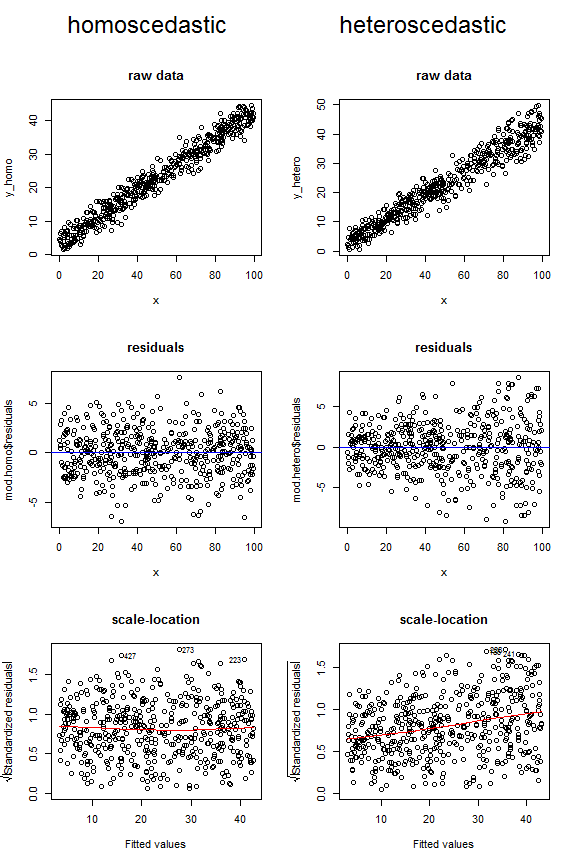
\includegraphics[width=0.7\linewidth]{homosked2.png}
\caption{}
\label{fig:homosked2}
\end{figure}
\newpage

%http://stats.stackexchange.com/questions/58141/interpreting-plot-lm
%\texttt{I explained the assumption of homoscedasticity and the plots that can help you assess it (including scale-location plots [2]) on CV here: What does having constant variance in a linear regression model mean? I have discussed qq-plots [3] on CV here: QQ plot does not match histogram. So, what's left is primarily just understanding [5], the residual-leverage plot.}


\newpage
\subsection{More Definitions}
To understand a diagnostic plot called the residual-leverage plot, we need to understand three things:

\begin{itemize}
	\item Leverage,
	\item Sstandardized residuals, and
	\item Cook's distance.
\end{itemize}
%Move next bit to "Leverarge"
\subsubsection{Leverage}
To understand leverage, recognize that \textit{Ordinary Least Squares} regression fits a line that will pass through the centre of your data, ($\bar{x}, \bar{y}$). The line can be shallowly or steeply sloped, but it will pivot around that point like a lever on a fulcrum. 

This analogy can be taken fairly literally: because OLS seeks to minimize the vertical distances between the data and the line, the data points that are further out towards the extremes of X will push / pull harder on the lever (i.e., the regression line); they have more leverage. One result of this could be that the results you get are driven by a few data points; that these diagnostic plots are intended to identify.

% Standardization
\subsubsection{Standardization}
Another result of the fact that points further out on X have more leverage is that they tend to be closer to the regression line (or more accurately: the regression line is fit so as to be closer to them) than points that are near $\bar{x}$. In other words, the residual standard deviation can differ at different points on X (even if the error standard deviation is constant). To correct for this, residuals are often standardized so that they have constant variance (assuming the underlying data generating process is homoscedastic, of course).

% Cook's Distance
\subsubsection{Cook's Distance}
One way to think about whether or not the results you have were driven by a given data point is to calculate how far the predicted values for your data would move if your model were fit without the data point in question. 

This calculated total distance is called \textbf{Cook's distance}. Fortunately, you don't have to rerun your regression model N times to find out how far the predicted values will move, Cook's D is a function of the leverage and standardized residual associated with each data point.

With these facts in mind, consider the plots associated with four different situations:
\begin{enumerate}
	\item a dataset where everything is fine
	\item a dataset with a high-leverage, but low-standardized residual point
	\item a dataset with a low-leverage, but high-standardized residual point
	\item a dataset with a high-leverage, high-standardized residual point
\end{enumerate}
\newpage
\begin{figure}[h!]
	\centering
	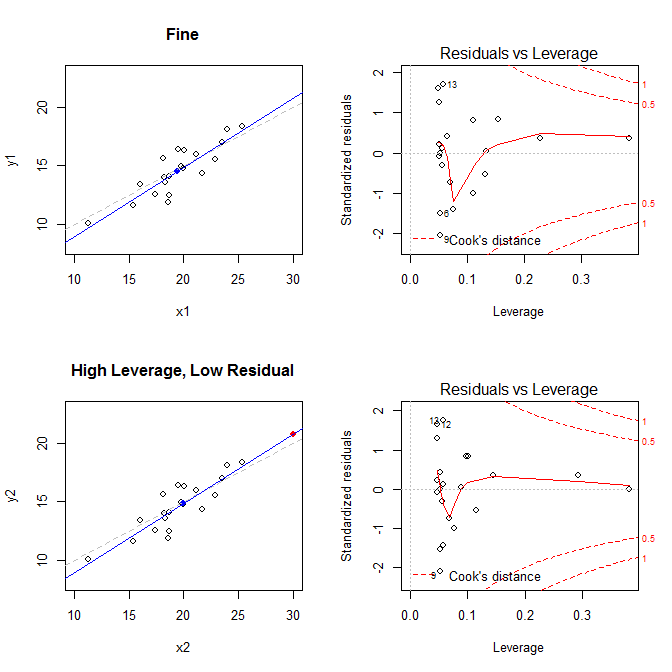
\includegraphics[width=1.0\linewidth]{plots2}
	\caption{}
	\label{fig:plots2}
\end{figure}
\newpage
\begin{figure}[h!]
\centering
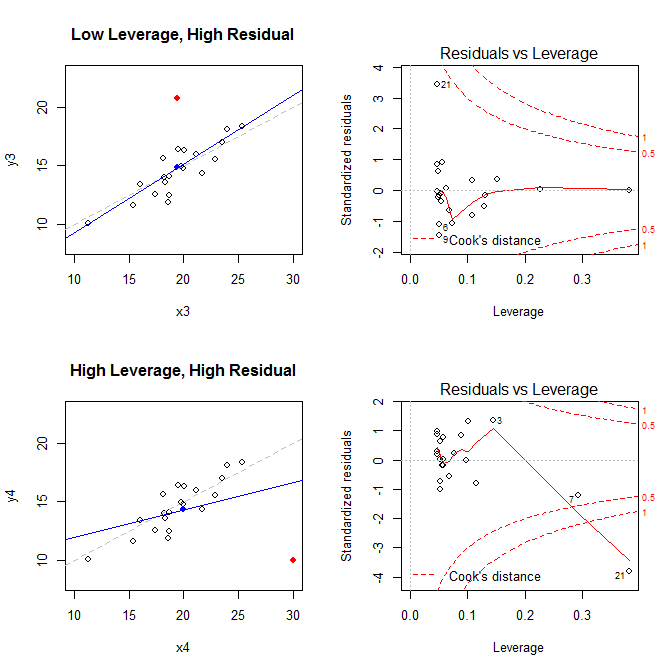
\includegraphics[width=1.0\linewidth]{plots3}
\caption{}
\label{fig:plots3}
\end{figure}
\newpage
\begin{itemize}
\item The plots on the left show the data, the center of the data  with a blue dot, the underlying data generating process with a dashed gray line, the model fit with a blue line, and the special point with a red dot. 
\item On the right are the corresponding residual-leverage plots; the special point is 21. 
\item The model is badly distorted primarily in the fourth case where there is a point with high leverage and a large (negative) standardized residual. 

\end{itemize}

%For reference, here are the values associated with the special points:

%                               leverage std.residual   cooks.d
%high leverage,  low residual  0.3814234    0.0014559 0.0000007
%low leverage,  high residual  0.0476191    3.4456341 0.2968102
%high leverage, high residual  0.3814234   -3.8086475 4.4722437
\end{document}